\renewcommand{\imglabel}[1]{\put(2,5){\tiny\contour{black}{\textcolor{white}{\textbf{#1}}}}}
\begin{figure}[!ht]
	\centering
	\setlength{\resLen}{0.12\columnwidth}	
	\addtolength{\tabcolsep}{-5pt}
	\begin{tabular}{ccccccccc}
		Photo & S1 & S2 & S3 & & Photo & S1 & S2 & S3
		\\
		\begin{overpic}[width=\resLen]{bayesian/fig7/1_bump_3/target.jpg}
			\imglabel{Bump-3}
		\end{overpic} &
		\includegraphics[width=\resLen]{bayesian/fig7/1_bump_3/good1.jpg} &
		\includegraphics[width=\resLen]{bayesian/fig7/1_bump_3/good2.jpg} &
		
\includegraphics[width=\resLen]{bayesian/fig7/1_bump_3/bad1.jpg} &
		&
		\begin{overpic}[width=\resLen]{bayesian/fig7/1_bump_4/target.jpg}
			\imglabel{Bump-4}
		\end{overpic} &
		\includegraphics[width=\resLen]{bayesian/fig7/1_bump_4/good1.jpg} &
		\includegraphics[width=\resLen]{bayesian/fig7/1_bump_4/good2.jpg} &
		
\includegraphics[width=\resLen]{bayesian/fig7/1_bump_4/bad1.jpg}
		\\
		\begin{overpic}[width=\resLen]{bayesian/fig7/2_leather_3/target.jpg}
			\imglabel{Leather-3}
		\end{overpic} &
		\includegraphics[width=\resLen]{bayesian/fig7/2_leather_3/good1.jpg} &
		\includegraphics[width=\resLen]{bayesian/fig7/2_leather_3/good2.jpg} &
		
\includegraphics[width=\resLen]{bayesian/fig7/2_leather_3/bad1.jpg} &
		&
		\begin{overpic}[width=\resLen]{bayesian/fig7/2_leather_4/target.jpg}
			\imglabel{Leather-4}
		\end{overpic} &
		\includegraphics[width=\resLen]{bayesian/fig7/2_leather_4/good1.jpg} &
		\includegraphics[width=\resLen]{bayesian/fig7/2_leather_4/good2.jpg} &
		
\includegraphics[width=\resLen]{bayesian/fig7/2_leather_4/bad1.jpg}
		\\
		\begin{overpic}[width=\resLen]{bayesian/fig7/2_leather_5/target.jpg}
			\imglabel{Leather-5}
		\end{overpic} &
		\includegraphics[width=\resLen]{bayesian/fig7/2_leather_5/good1.jpg} &
		\includegraphics[width=\resLen]{bayesian/fig7/2_leather_5/good2.jpg} &
		
\includegraphics[width=\resLen]{bayesian/fig7/2_leather_5/bad1.jpg} &
		&
		\begin{overpic}[width=\resLen]{bayesian/fig7/2_leather_6/target.jpg}
			\imglabel{Leather-6}
		\end{overpic} &
		\includegraphics[width=\resLen]{bayesian/fig7/2_leather_6/good1.jpg} &
		\includegraphics[width=\resLen]{bayesian/fig7/2_leather_6/good2.jpg} &
		
\includegraphics[width=\resLen]{bayesian/fig7/2_leather_6/bad1.jpg}
		\\
		\begin{overpic}[width=\resLen]{bayesian/fig7/3_plaster_3/target.jpg}
			\imglabel{Plaster-3}
		\end{overpic} &
		\includegraphics[width=\resLen]{bayesian/fig7/3_plaster_3/good1.jpg} &
		\includegraphics[width=\resLen]{bayesian/fig7/3_plaster_3/good2.jpg} &
		
\includegraphics[width=\resLen]{bayesian/fig7/3_plaster_3/bad1.jpg} &
		&
		\begin{overpic}[width=\resLen]{bayesian/fig7/3_plaster_4/target.jpg}
			\imglabel{Plaster-4}
		\end{overpic} &
		\includegraphics[width=\resLen]{bayesian/fig7/3_plaster_4/good1.jpg} &
		\includegraphics[width=\resLen]{bayesian/fig7/3_plaster_4/good2.jpg} &
		
\includegraphics[width=\resLen]{bayesian/fig7/3_plaster_4/bad1.jpg}
		\\
		\begin{overpic}[width=\resLen]{bayesian/fig7/4_flake_3/target.jpg}
			\imglabel{Metallicflake-3}
		\end{overpic} &
		\includegraphics[width=\resLen]{bayesian/fig7/4_flake_3/good1.jpg} &
		\includegraphics[width=\resLen]{bayesian/fig7/4_flake_3/good2.jpg} &
		
\includegraphics[width=\resLen]{bayesian/fig7/4_flake_3/bad1.jpg} &
		&
		\begin{overpic}[width=\resLen]{bayesian/fig7/4_flake_4/target.jpg}
			\imglabel{Metallicflake-4}
		\end{overpic} &
		\includegraphics[width=\resLen]{bayesian/fig7/4_flake_4/good1.jpg} &
		\includegraphics[width=\resLen]{bayesian/fig7/4_flake_4/good2.jpg} &
		
\includegraphics[width=\resLen]{bayesian/fig7/4_flake_4/bad1.jpg}
		\\
		\begin{overpic}[width=\resLen]{bayesian/fig7/5_metal_3/target.jpg}
			\imglabel{Brushmetal-3}
		\end{overpic} &
		\includegraphics[width=\resLen]{bayesian/fig7/5_metal_3/good1.jpg} &
		\includegraphics[width=\resLen]{bayesian/fig7/5_metal_3/good2.jpg} &
		
\includegraphics[width=\resLen]{bayesian/fig7/5_metal_3/bad1.jpg} &
		&
		\begin{overpic}[width=\resLen]{bayesian/fig7/6_wood_3/target.jpg}
			\imglabel{Wood-3}
		\end{overpic} &
		\includegraphics[width=\resLen]{bayesian/fig7/6_wood_3/good1.jpg} &
		\includegraphics[width=\resLen]{bayesian/fig7/6_wood_3/good2.jpg} &
		
\includegraphics[width=\resLen]{bayesian/fig7/6_wood_3/bad1.jpg}
		\\
		\begin{overpic}[width=\resLen]{bayesian/fig7/6_wood_4/target.jpg}
			\imglabel{Wood-4}
		\end{overpic} &
		\includegraphics[width=\resLen]{bayesian/fig7/6_wood_4/good1.jpg} &
		\includegraphics[width=\resLen]{bayesian/fig7/6_wood_4/good2.jpg} &
		
\includegraphics[width=\resLen]{bayesian/fig7/6_wood_4/bad1.jpg} &
		&
		\begin{overpic}[width=\resLen]{bayesian/fig7/6_wood_5/target.jpg}
			\imglabel{Wood-5}
		\end{overpic} &
		\includegraphics[width=\resLen]{bayesian/fig7/6_wood_5/good1.jpg} &
		\includegraphics[width=\resLen]{bayesian/fig7/6_wood_5/good2.jpg} &
		
\includegraphics[width=\resLen]{bayesian/fig7/6_wood_5/bad1.jpg}
	\end{tabular}
	\caption[Real results]{\label{fig:bayesian:real}
		\textbf{Results} of our MCMC sampling on \textbf{real} inputs. For each example, the first column is the real target image (photo). We show MCMC samples in the other columns, where sample-1 and sample-2 are chosen closer to the peak of the posterior distribution, and sample-3 is further away. Note that the target images for Plaster-4 and Wood-5 are captured under natural illumination, while the corresponding synthetic images still assume collocated flash illumination; despite this mismatch, the estimated material parameters are still reasonable. Note, target images for Leather-4, Leather-6 and Wood-4 are from the publicly released dataset of \cite{aittala2016reflectance}. For more results please refer to supplemental materials.
	}
\end{figure}
